\section{Mediciones}

Se realizaron mediciones en base a crear sets de distinta cantidad de
elementos, con la cantidad de subsets y la cantidad de elementos por subset
siendo proporcional a la cantidad de elementos.

Para asegurar la validez de las comparaciones todas las mediciones fueron
realizadas sobre los mismos sets de datos para los métodos que están siendo
comparados. Los elementos fueron generados por los valores pseudoaleatorios del
lenguaje (el módulo \texttt{random}) con la misma \textit{seed}.

\subsection{Backtracking vs. Programación Lineal}

\begin{figure}[H]
    \centering
    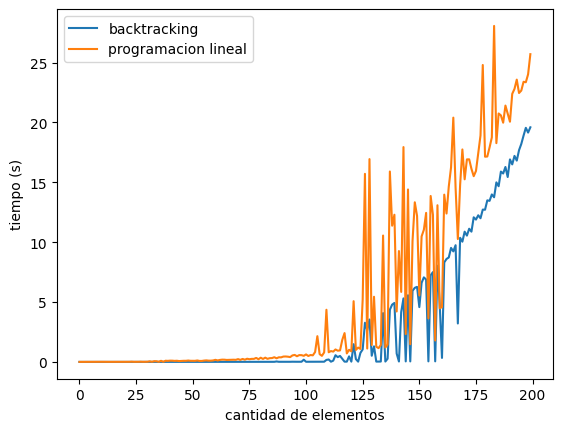
\includegraphics[width=1\textwidth]{img/backvslp.png}
\end{figure}

Backtracking obtiene mejores tiempo de ejecución que programación lineal para
encontrar la solución óptima.

\subsection{Algoritmos de aproximación}

\begin{figure}[H]
    \centering
    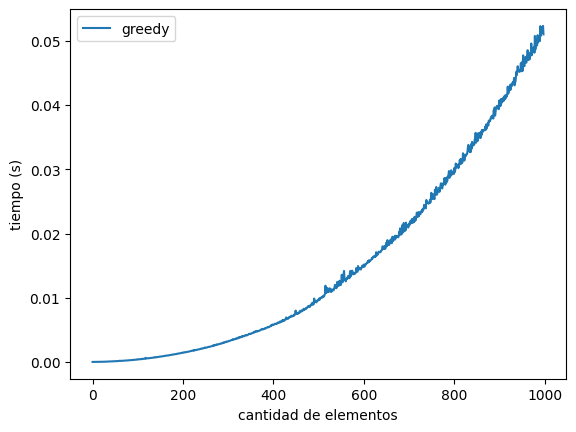
\includegraphics[width=0.49\textwidth]{img/greedy.png}
    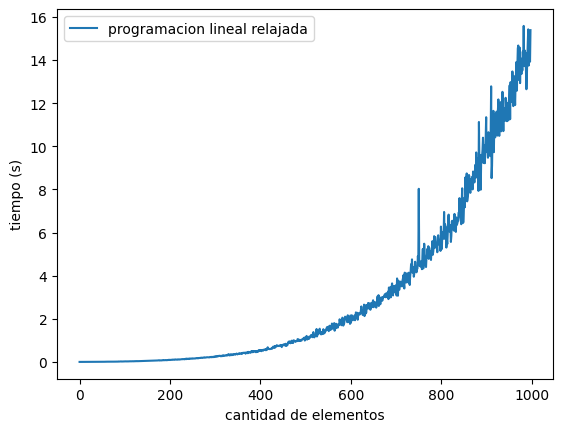
\includegraphics[width=0.49\textwidth]{img/pl_rlx.png}
\end{figure}

Notar la diferencia de tiempos (eje y) entre greedy y programación lineal.

\subsubsection{Calidad de las aproximaciones}

Si comparamos el tamaño de la solución que obtenemos utilizando cada algoritmo,
vemos que el algoritmo greedy provee mejores soluciones que el algoritmo por
programación lineal relajada, y que dichas soluciones no se alejan mucho del
óptimo.

\begin{figure}[H]
    \centering
    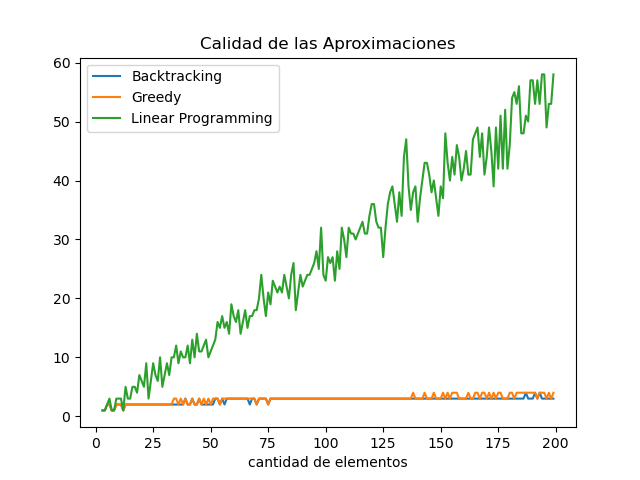
\includegraphics[width=1\textwidth]{img/quality.png}
\end{figure}

\subsubsection{Mejoras al algoritmo por programación lineal relajada}

Dado que las soluciones por programación lineal relajada estan tan lejos del
óptimo, proponemos una mejora al algoritmo. Luego de obtener el valor en el
óptimo de las variables, tomamos la variable de mayor valor de cada subset,
priorizando las variables que ya forman parte de la solución, esta aproximación
es por lo menos tan bueno como la aproximación utilizada anteriormente porque
el valor de la variable con mayor valor de cada subset siempre es mayor o igual
a $\frac{1}{b}$, por lo que también forma parte de la solución vieja.

\begin{figure}[H]
    \centering
    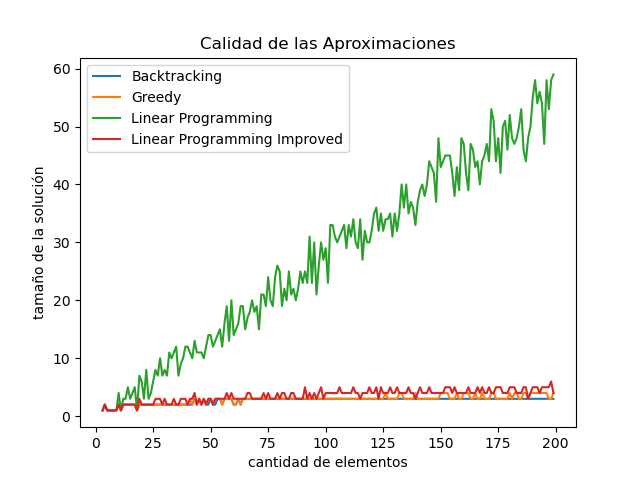
\includegraphics[width=1\textwidth]{img/quality2.png}
\end{figure}

\newpage

\subsection{Cota de la relajación lineal}

Se realizaron mediciones para verificar la cota calculada empiricamente con un
valor de $r(A) = 20$:

\begin{figure}[H]
    \centering
    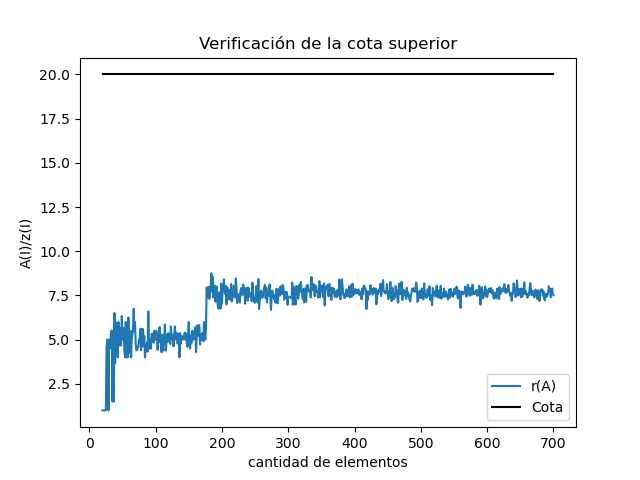
\includegraphics[width=0.8\textwidth]{img/cota.png}
\end{figure}

Vemos que $\frac{A(I)}{z(I)}$ se mantiene por debajo de la cota calculada. Cabe
aclarar que a partir de los 175 elementos se utilizó una cota inferior para
$z(I)$, por lo que se ve un pico en el gráfico a partir de ahí, esta cota
inferior fue calculada por el mismo algoritmo de programación lineal relajada
porque los volumenes de datos eran inmanejables para el algoritmo exacto.
